\documentclass[11pt, a4paper]{article}
\usepackage[utf8]{inputenc}
\usepackage{minted}
\usepackage{graphicx}
\graphicspath{{./images/}}

\usepackage{hyperref}

\title{Advanced Lane Line Finding}
\author{Samuel Navarro}
\date{\today}

\begin{document}
\maketitle

\tableofcontents{}



\section{Camera Calibration}
\label{sec:camera_calibration}

The code for this step is implemented in the third and fourth cell of the jupyter notebook in the functions \texttt{show\_image} and \texttt{calibrate\_camera}. 

The output of \texttt{calibrate\_camera} gives us the objpoints and the imgpoints arrays. I then use the this arrays to obtain the distortion coefficients and the camera matrix to obtain the undistorted image. 

An example is in the Figure 1 and 2~\ref{fig:undistort} 


\begin{figure}[htb!]
    \centering
    \begin{minipage}{0.5\textwidth}
        \centering
		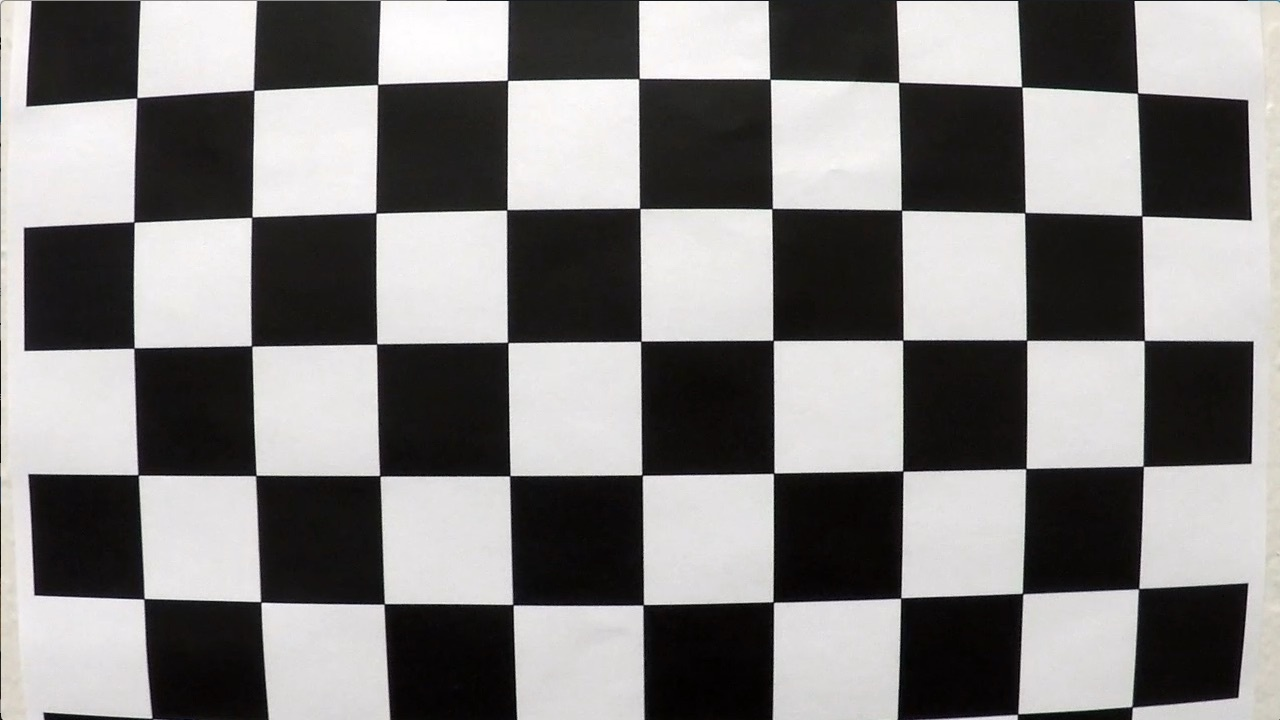
\includegraphics[width=1\textwidth]{chess_img} 
        \caption{Original}
		\label{fig:original_chess}
    \end{minipage}\hfill
    \begin{minipage}{0.5\textwidth}
        \centering
		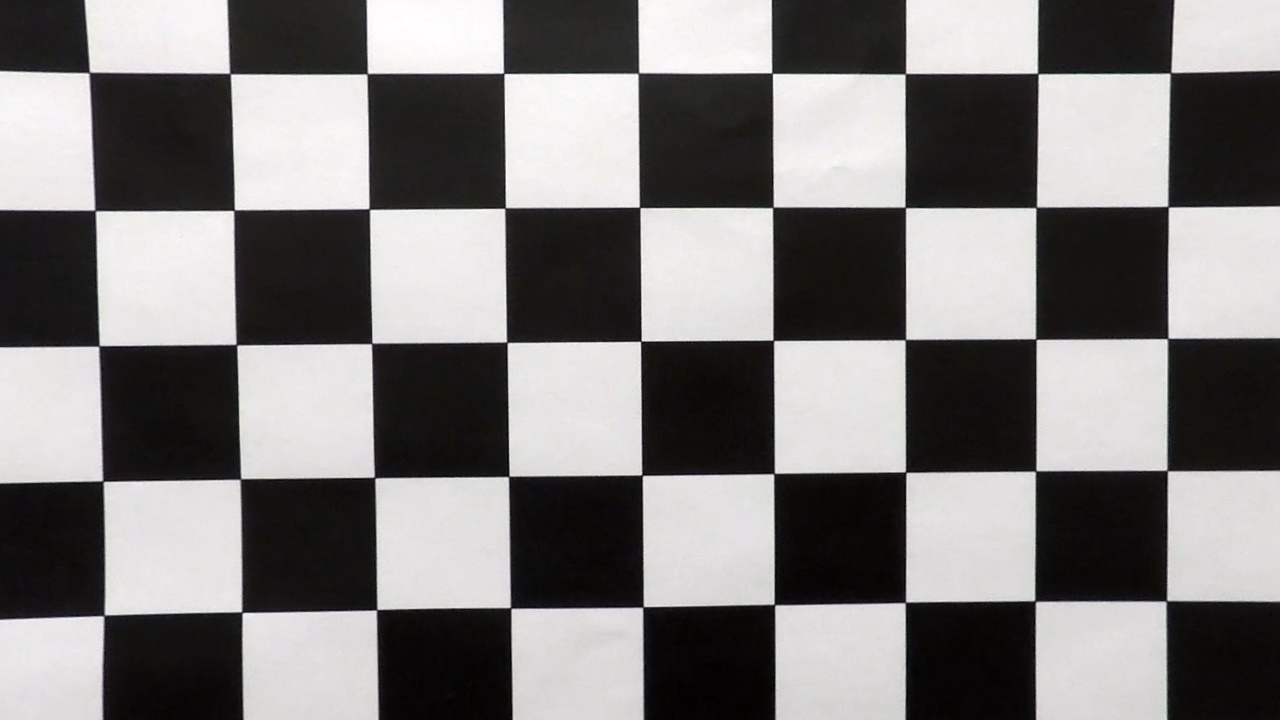
\includegraphics[width=1\textwidth]{undistorted_chess} 
        \caption{Undistorted}
		\label{fig:undistorted_chess}
    \end{minipage}
	\label{fig:undistort}
\end{figure}


\section{Pipeline Images}
\label{sec:pipeline_images}

\subsection{Undistorted test}%
\label{sub:undistorted_test}


We can se te distortion correction being applied in one of the test images:

\begin{figure}[htb!]
	\centering
	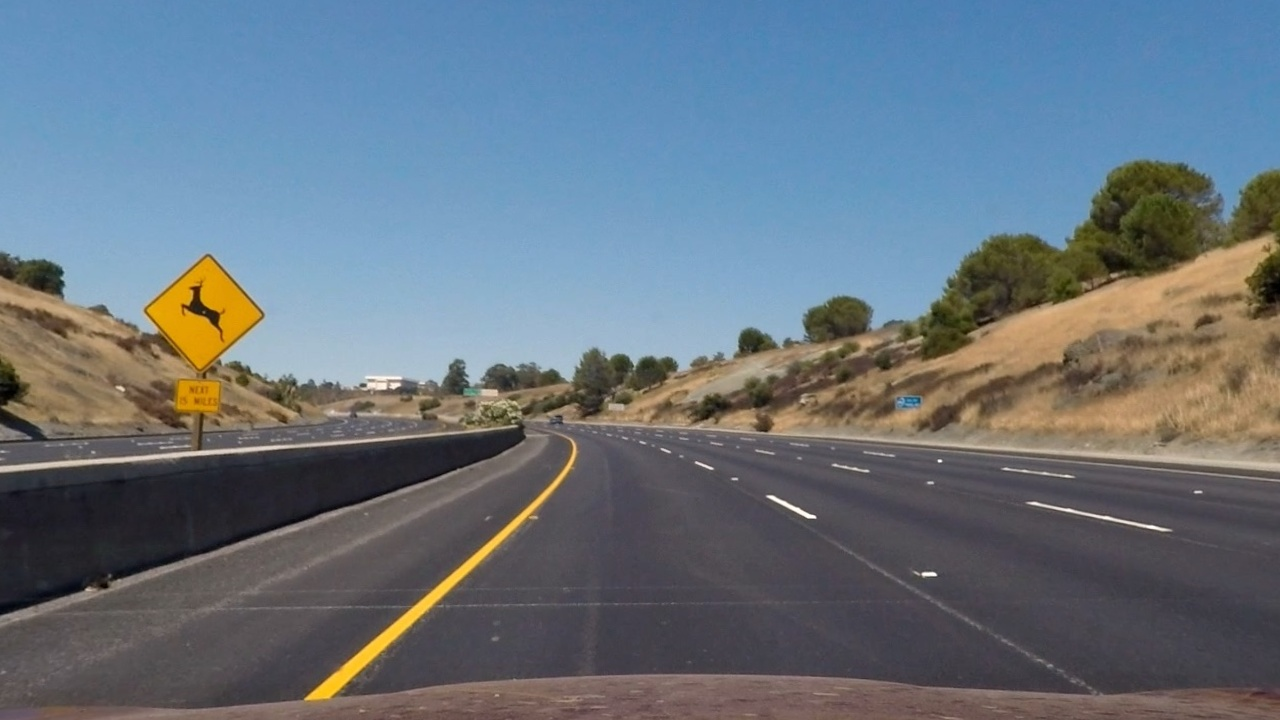
\includegraphics[width=0.8\linewidth]{undist}
	\caption{Undistorted test}
	\label{fig:undistorted_test}
\end{figure}

\subsection{Perspective Transform}%
\label{sub:perspective_transform}

The perspective transform is in the function \texttt{perspective\_transform} in the same notebook.

The parameters I used was hardcoded. This is obviously something that can be improved. The most straightforward way I can think of based on what we've learned is applying Hough Transform in the image and apply the perspective transform on that. 

The result is in the Figure~\ref{fig:warped}:


\begin{figure}[htb!]
	\centering
	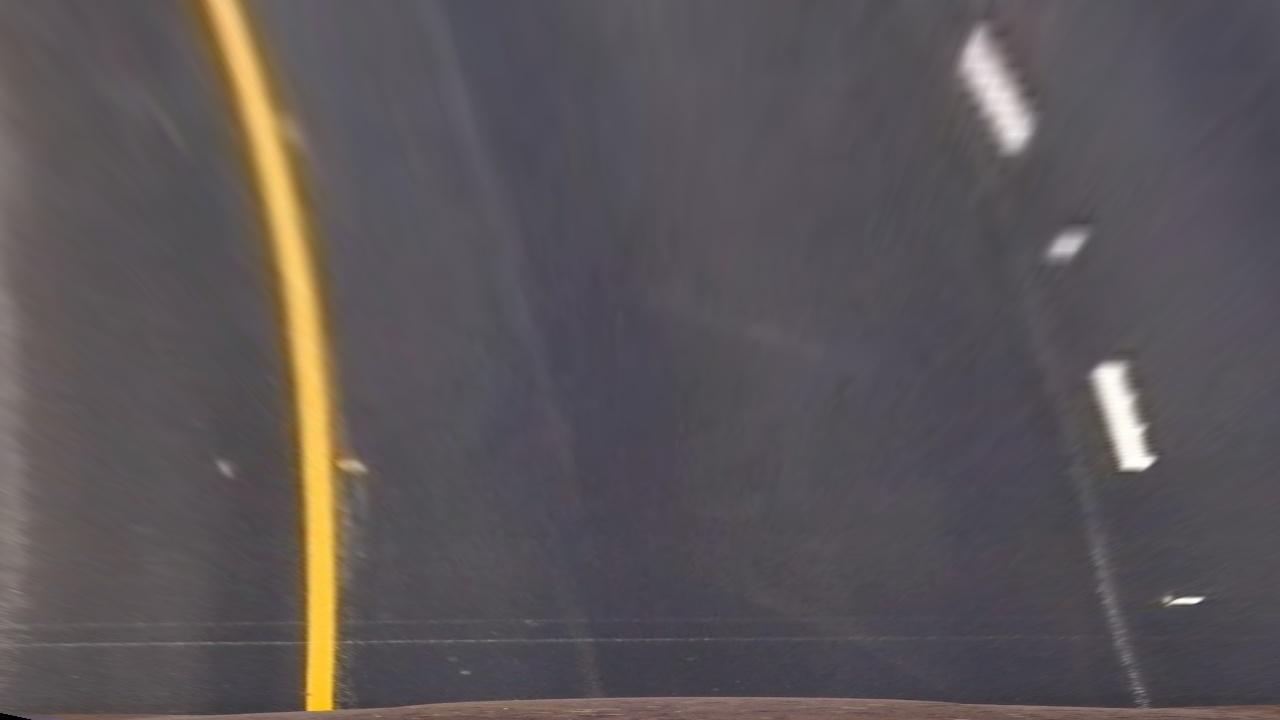
\includegraphics[width=0.8\linewidth]{warped}
	\caption{Warped}
	\label{fig:warped}
\end{figure}




\subsection{Color transforms and gradients}%
\label{sub:color_transforms_and_gradients}


Then, with the warped image at hand, I used a combination of color and gradient thresholds. The code is in the function \texttt{color\_pipeline}.


I figure out that when the road is clear, the s\_channel is better to find the lanes but when the road is dark because of some shadow caused by the threes, the l\_channel was better. 

Because of that, I used a combination l and s channel images with and without x gradient.

The result can be found in the Figure~\ref{fig:combined_binary}



\begin{figure}[htb!]
	\centering
	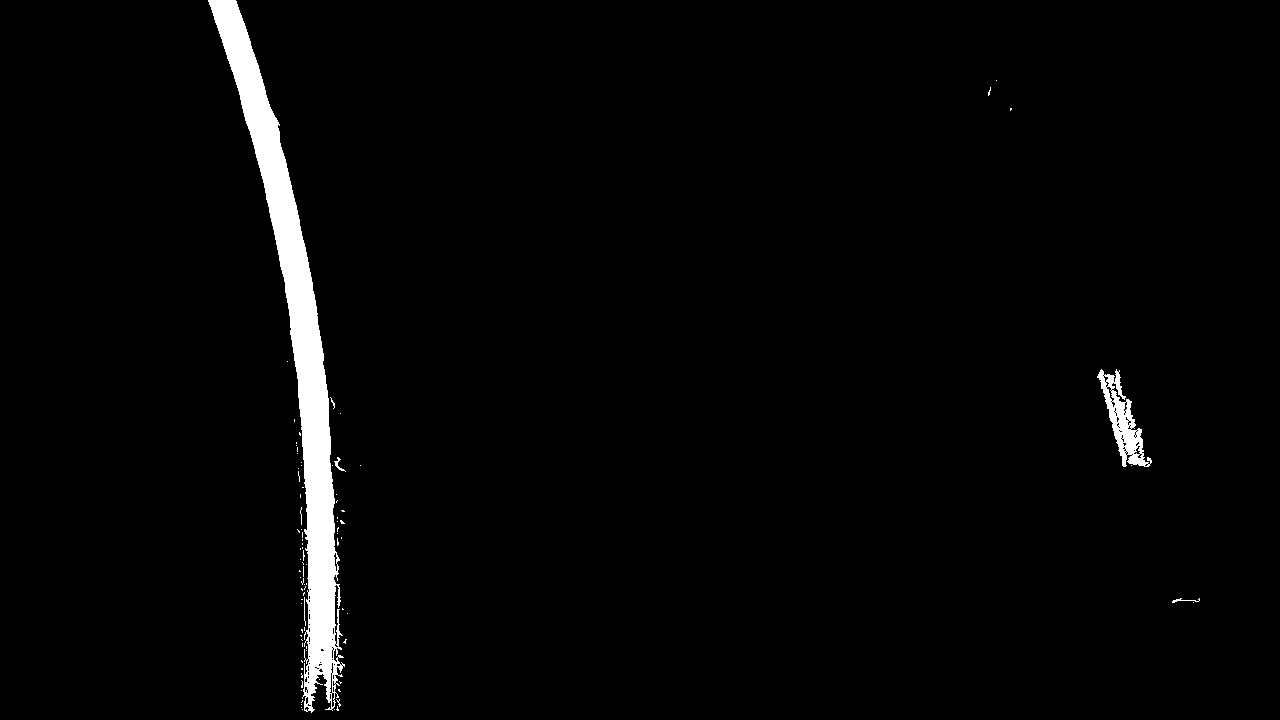
\includegraphics[width=0.8\linewidth]{combined_binary}
	\caption{Combined Binary}
	\label{fig:combined_binary}
\end{figure}




\subsection{Fitted Lane Lines}%
\label{sub:fitted_lane_lines}

The functions I used to fit the lines was \texttt{search\_around\_poly}. The result can be found in the Figure~\ref{fig:fitted_lines}.




For the video I used the \texttt{search\_around\_poly} but for illustration I used the \texttt{old\_search\_around\_poly} function to illustrate the windows. 

\begin{figure}[htb!]
	\centering
	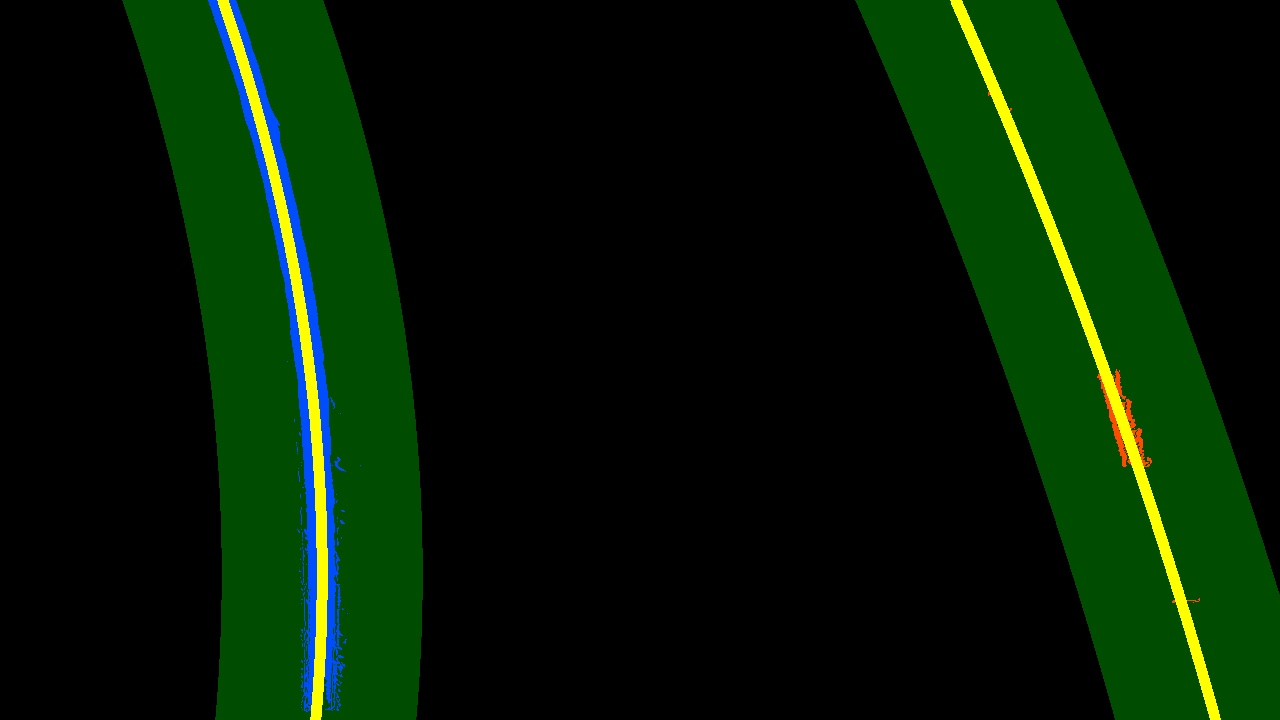
\includegraphics[width=0.8\linewidth]{fitted_lines}
	\caption{Fitted Lines}
	\label{fig:fitted_lines}
\end{figure}










\section{Discussion}
\label{sec:discussion}



\begin{itemize}
	\item One of the problems I encounter was the fact that you have a difference in the frames when you are trying to diagnose the problems. It seems obvious when you know you are dealing with the undistorted frames but at the beginning I was trying to diagnose the problems with the original frame.
\end{itemize}


One of the things I believed I could make different was to make a moving window to detect the lines. I believed that you can make a mask of the image in places where you got peaks in your histogram.

But, this approach could be more computationally expensive because you have to use `cv2.fitPoly`. The fact that the parameters of `cv2.rectangle` are just two points makes it easy also to draw the rectangles.






\end{document}
